\section{问题二：变物性双向强耦合下的全过程温度与水分场}\label{sec:p2}

\subsection{相对问题一的增量：变物性与双向耦合}

问题二保留问题一的柱坐标控制方程~\eqref{eq:pde} 与恒定热风，但把附录2 常物性替换为附录3
变物性：$\rho=650+128C$、$c_p=1450+2736\frac{C}{C+1}$、$k=0.21+0.38\frac{C}{C+1}$，扩散系数按
式~\eqref{eq:diff} 取 $D_0=2.4\times10^{-3},a=0.45$。此时含水率 $C$ 通过 $\rho,c_p,k$ 影响温度场，
温度 $T$ 又通过 Arrhenius 项 $\exp(-E/T_K)$ 影响扩散、进而改变含水率，构成\textbf{双向强耦合}。
求解时 $T,C$ 在同一 Picard 回路内联立更新（式~\eqref{eq:picard}），观测时窗取 $0\sim3\,\mathrm{h}$。

\subsection{结果与分析}

图~\ref{fig:field_heatmap_p2} 给出含水率场的时空演化与边缘剖面。

\begin{figure}[H]
  \centering
  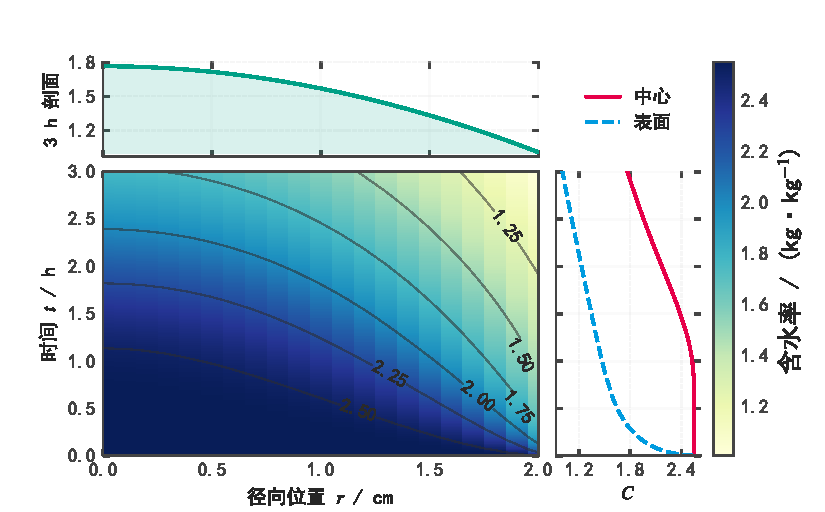
\includegraphics[width=0.9\textwidth,height=0.8\textheight,keepaspectratio]{../figures/fig_field_heatmap_p2.pdf}
  \caption{问题2 含水率场时空演化与不同时刻的边缘剖面}
  \label{fig:field_heatmap_p2}
\end{figure}

由图~\ref{fig:field_heatmap_p2}，$3\,\mathrm{h}$ 时轴心含水率降至 $1.7662$、表面降至 $1.0078$，
沿半径由轴心到表面为 $1.7662$,\allowbreak\,$1.7165$,\allowbreak\,$1.5701$,\allowbreak\,$1.3331$,\allowbreak\,$1.0078$（对应问题2 剖面见
图~\ref{fig:radial_profiles} 右）；与问题一相比，失水已从表面薄层推进到全径，但\textbf{距阈值
$0.15$ 仍有量级差距}，说明 $3\,\mathrm{h}$ 远未达标，为问题三的长时程计算埋下伏笔。温度场
等值线见图~\ref{fig:temp_contour_p2}。

\begin{figure}[H]
  \centering
  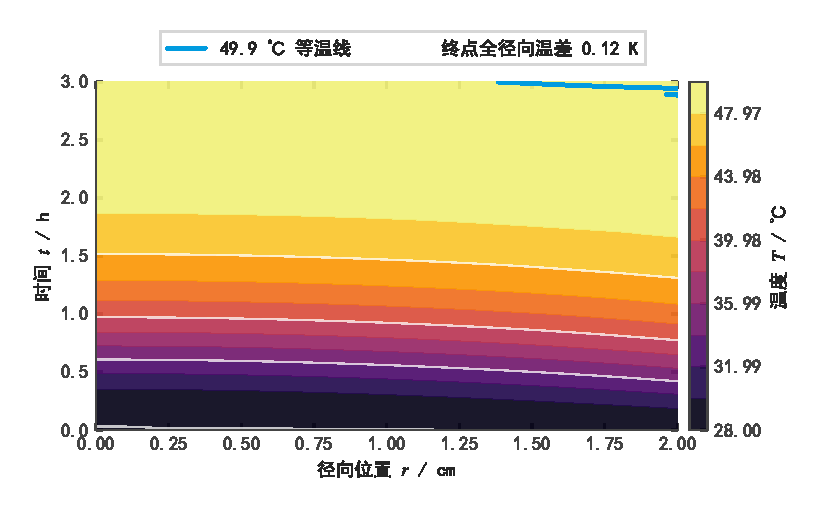
\includegraphics[width=0.9\textwidth,height=0.8\textheight,keepaspectratio]{../figures/fig_temp_contour_p2.pdf}
  \caption{问题2 温度场等值线与 $49.9\,^{\circ}\mathrm{C}$ 等温线}
  \label{fig:temp_contour_p2}
\end{figure}

图~\ref{fig:temp_contour_p2} 显示 $3\,\mathrm{h}$ 时温度场已近乎均匀：沿半径为
$49.8495$,\allowbreak\,$49.8554$,\allowbreak\,$49.8746$,\allowbreak\,$49.9101$,\allowbreak\,$49.9664\,^{\circ}\mathrm{C}$，全场温差不足 $0.12\,^{\circ}\mathrm{C}$，
$49.9\,^{\circ}\mathrm{C}$ 等温线已逼近轴心，表明\textbf{温度场早已进入准稳态，而含水率场仍在缓慢演化}。
这一"热快质慢"的分离是本题的核心机理，定量刻画见图~\ref{fig:timescale_split}。

\begin{figure}[H]
  \centering
  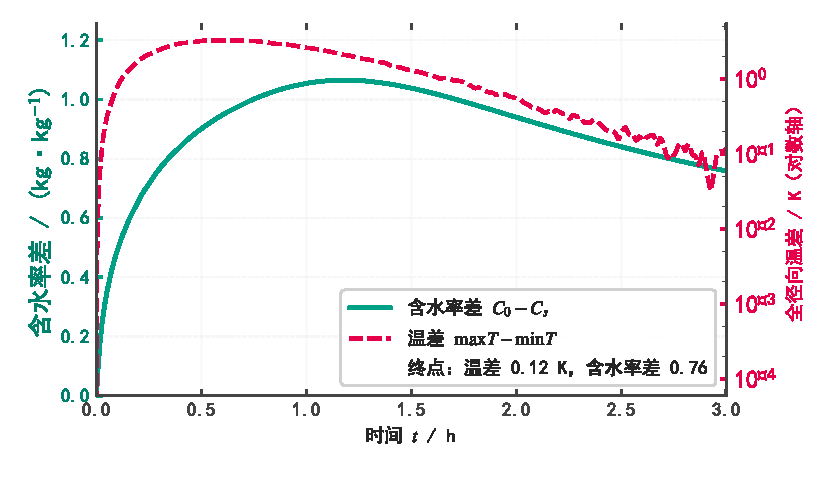
\includegraphics[width=0.9\textwidth,height=0.8\textheight,keepaspectratio]{../figures/fig_timescale_split.pdf}
  \caption{问题2 传热与传质特征时间尺度的分离}
  \label{fig:timescale_split}
\end{figure}

图~\ref{fig:timescale_split} 比较传热与传质的特征时间：传质时间与传热时间之比
$\tau_m/\tau_{\mathrm{th}}$ 由初始约 $30$ 增大到终点约 $211$，即水分迁移比热量传递慢一到两个数量级，
且随含水率下降差距进一步拉大。这解释了为何可以近似认为温度场先达稳态、再驱动缓慢的
失水过程，也为问题三只在含水率场上设终点判据（而非温度场）提供了尺度依据。
